\documentclass[../notes.tex]{subfiles}

\pagestyle{main}
\renewcommand{\chaptermark}[1]{\markboth{\chaptername\ \thechapter\ (#1)}{}}
\setcounter{chapter}{4}

\begin{document}




\chapter{Non-Inertial Reference Frames}
\section{Rotating Reference Frames}
\begin{itemize}
    \item \marginnote{10/23:}Recap: Scattering.
    \begin{itemize}
        \item For a particular central force, we can find $b(\Theta)$.
        \item The differential cross-section (what is this??).
        \item For a general potential $V(r)$, we can use the orbit equation to solve for the angular change from $r_\text{min}$ to $r_\text{max}$ and back.
        \begin{itemize}
            \item The "and back" part is why we get the 2 coefficient!
            \item HW: Use this to derive a general relationship $b(\Theta)$ for any $V$.
        \end{itemize}
        \item For a \textbf{closed}, non-circular orbit, we must have integers $a,b$ such that
        \begin{equation*}
            2\pi = \Delta\theta\cdot\frac{a}{b}
        \end{equation*}
        \begin{itemize}
            \item Curiously, for $V(r)=kr^{n+1}$, only $n=1$ (attractive harmonic oscillator) and $n=-2$ (inverse square law) have this property!
            \item Does she mean $n=-1$ if we're talking about inverse square law \emph{potential}?? Also, need for what??
        \end{itemize}
    \end{itemize}
    \item Today.
    \begin{itemize}
        \item Rotating reference frames.
        \item Gravity + Coriolis Effect.
    \end{itemize}
    \item \textbf{Vector angular velocity}: The vector defined as follows, which describes the angular velocity of a rotating body. \emph{Denoted by} $\bm{\vec{\omega}}$. \emph{Given by}
    \begin{equation*}
        \vec{\omega} = \omega\khat
    \end{equation*}
    \item Example:
    \begin{equation*}
        \omega_\text{earth} = \frac{2\pi}{\SI{24}{\hour}}
        = \SI{7.3e-5}{\per\second}
    \end{equation*}
    \item Define vectors $\ihat,\jhat,\khat$ that \emph{rotate} about $\khat$ to remain fixed on the surface of the rotating body.
    \item For a fixed vector $\hat{r}$ on a rotating body, the change in $\vec{r}$ with respect to time according to an inertial observer is given by
    \begin{equation*}
        \dv{\vec{r}}{t} = \vec{v}
        = \vec{\omega}\times\vec{r}
    \end{equation*}
    \begin{figure}[h!]
        \centering
        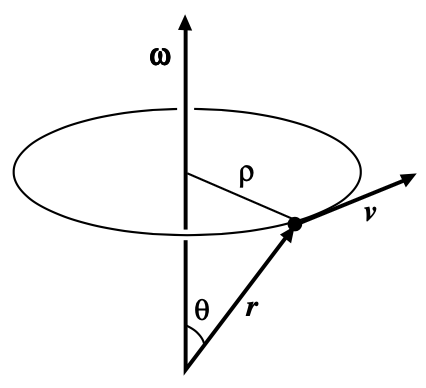
\includegraphics[width=0.25\linewidth]{../ExtFiles/Vrotation.png}
        \caption{Rotational velocity.}
        \label{fig:Vrotation}
    \end{figure}
    \begin{itemize}
        \item Proof: $v=\omega\rho=r\omega\sin\theta$.
    \end{itemize}
    \item The specific case where $\vec{r}=\ihat,\jhat,\khat$.
    \begin{align*}
        \dv{\ihat}{t} &= \vec{\omega}\times\ihat&
        \dv{\jhat}{t} &= \vec{\omega}\times\jhat&
        \dv{\khat}{t} &= \vec{\omega}\times\khat
    \end{align*}
    \item The case where the vector is time-dependent.
    \begin{itemize}
        \item Let $\vec{b}=b_x\ihat+b_y\jhat+b_z\khat$, where $b_x,b_y,b_z$ are functions of time.
        \item Define notions of \textbf{absolute} and \textbf{relative} velocity.
        \item Relationship between the above two quantities:
        \begin{align*}
            \dv{\vec{b}}{t} &= (\dot{b}_x\ihat+\dot{b}_y\jhat+\dot{b}_z\khat)+\left( b_x\dv{\ihat}{t}+b_y\dv{\jhat}{t}+b_z\dv{\khat}{t} \right)\\
            &= \dot{\vec{b}}+b_x\vec{\omega}\times\ihat+b_y\vec{\omega}\times\jhat+b_z\vec{\omega}\times\khat\\
            &= \dot{\vec{b}}+\vec{\omega}\times\vec{b}
        \end{align*}
        \item The last line above is definitely worth remembering.
    \end{itemize}
    \item \textbf{Absolute} (velocity): The time rate of change of $\vec{r}$ as observed in an \emph{inertial} frame. \emph{Denoted by} $\bm{\textbf{d}\vec{r}/\textbf{d}t}$, $\bm{\vec{v}_\textbf{inertial observer}}$, $\bm{\vec{v}}$. \emph{Given by}
    \begin{equation*}
        \dv{\vec{r}}{t} = \dot{\vec{r}}+\vec{\omega}\times\vec{r}
    \end{equation*}
    \item \textbf{Relative} (velocity): The time rate of change of $\vec{r}$ as observed in a \emph{rotating} frame. \emph{Denoted by} $\bm{\dot{\vec{r}}}$. \emph{Given by}
    \begin{equation*}
        \dot{\vec{r}} = \dot{r}_x\ihat+\dot{r}_y\jhat+\dot{r}_z\khat
    \end{equation*}
    \item \textbf{Absolute} (acceleration): The time rate of change of $\vec{v}_\text{inertial observer}$ as observed in an \emph{inertial} frame. \emph{Denoted by} $\bm{\textbf{d}\vec{v}/\textbf{d}t}$, $\bm{\vec{a}_\textbf{inertial observer}}$, $\bm{\textbf{d}^2\vec{r}/\textbf{d}t^2}$. \emph{Given by}
    \begin{equation*}
        \dv{\vec{v}}{t} = \dot{\vec{v}}+\vec{\omega}\times\vec{v}
    \end{equation*}
    \item \textbf{Relative} (acceleration): The time rate of change of $\vec{v}_\text{inertial observer}$ as observed in a \emph{rotating} frame. \emph{Denoted by} $\bm{\dot{\vec{v}}}$. \emph{Given by}
    \begin{equation*}
        \dot{\vec{v}} = \ddot{\vec{r}}+\vec{\omega}\times\dot{\vec{r}}
    \end{equation*}
    \begin{itemize}
        \item Note that this result only holds when $\vec{\omega}$ is constant.
    \end{itemize}
    \item Let's investigate the $\vec{\omega}\times\vec{v}$ from the definition of absolute acceleration a bit more closely.
    \begin{itemize}
        \item Substituting in the definition of $\vec{v}$ as $\dot{\vec{r}}+\vec{\omega}\times\vec{r}$, we obtain
        \begin{equation*}
            \vec{\omega}\times\vec{v} = \vec{\omega}\times\dot{\vec{r}}+\vec{\omega}\times(\vec{\omega}\times\vec{r})
        \end{equation*}
        \item Thus, we can alternatively write an expression for absolute acceleration as follows.
        \begin{equation*}
            \dv[2]{\vec{r}}{t} = \ddot{\vec{r}}+2\vec{\omega}\times\dot{\vec{r}}+\vec{\omega}\times(\vec{\omega}\times\vec{r})
        \end{equation*}
        \item This last term points toward the axis of rotation.
        \begin{itemize}
            \item See \textcite{bib:KibbleBerkshire}, Q5.19, for more.
        \end{itemize}
    \end{itemize}
    \item Using the above discussion and result, we will analyze physics near Earth's surface.
    \begin{itemize}
        \item For a particle moving under gravity $m\vec{g}=-GMm/R^2\approx 9.81m$ and under other, additional forces $\vec{F}$, the equation of motion is
        \begin{equation*}
            m\vec{a}_\text{inertial} = m\vec{g}+\vec{F}
        \end{equation*}
        \item What we measure on earth is $m\ddot{\vec{r}}$. It is related to the above quantities via the result from the previous discussion as follows.
        \begin{equation*}
            m\ddot{\vec{r}} = m\vec{g}+\vec{F}-2m\vec{\omega}\times\dot{\vec{r}}-m\vec{\omega}\times(\vec{\omega}\times\vec{r})
        \end{equation*}
        \begin{itemize}
            \item Note that the $-2m\vec{\omega}\times\dot{\vec{r}}$ and $-m\vec{\omega}\times(\vec{\omega}\times\vec{r})$ terms are known as the \textbf{Coriolis} and \textbf{centrifugal} forces, respectively.
            \item These forces are "apparent" or "fictitious" forces caused by our rotational motion; they are not \emph{actual} forces like pushing on something.
        \end{itemize}
    \end{itemize}
    \item Consider a particle that is not under the influence of any force besides gravity (e.g., a projectile).
    \begin{itemize}
        \item Suppose it lies at latitude $\pi/2-\theta$ and longitude $\phi$.
        \item Refresher: On Earth, $\vec{\omega}=\omega\khat$.
        \item There are three local coordinates on Earth's surface: \textbf{East} ($\hat{e}$), \textbf{north} ($\hat{n}$), and \textbf{up} ($\hat{r}$).
        \begin{itemize}
            \item Note that naturally, up shares a symbol with the radial vector because they both point in the same direction: Away from the center of the Earth/spherical body in question.
        \end{itemize}
        \item Note: From trigonometry,
        \begin{equation*}
            \vec{\omega} = \omega\cos\theta\hat{r}+\omega\sin\theta\hat{n}
        \end{equation*}
        \begin{itemize}
            \item It follows that the $\hat{r}$ component of $\vec{\omega}$ is inwards in the southern hemisphere!
        \end{itemize}
        \item Thus, in terms of all of these local coordinates, the relative acceleration of the particle can be described as follows.
        \begin{equation*}
            \ddot{\vec{r}} = -g\hat{r}-2\omega(\cos\theta\hat{r}+\sin\theta\hat{n})\times(\dot{r}_r\hat{r}+\dot{r}_e\hat{e}+\dot{r}_n\hat{n})-\omega^2R\sin\theta(-\sin\theta\hat{r}+\cos\theta\hat{n})
        \end{equation*}
        \begin{itemize}
            \item Note that the last term comes from expanding $(\omega\cos\theta\hat{r}+\omega\sin\theta\hat{n})\times[(\omega\cos\theta\hat{r}+\omega\sin\theta\hat{n})\times R\hat{r}]$. We take $\vec{r}=R\hat{r}$ here because we are using polar coordinates, not $\ihat,\jhat,\khat$.
        \end{itemize}
        \item Using the $\hat{r}$ component of the above, we can reconstruct the gravitational force at Earth's surface.
        \begin{equation*}
            \ddot{r}_r = -g+2\omega\sin\theta\dot{r}_e+\omega^2R\sin^2\theta
            \approx -g
        \end{equation*}
        \begin{itemize}
            \item We say that the sum of the three terms above is approximately equal to the first term because the first term is 2-5 orders of magnitude larger than the other two ($\omega=\SI{7.3e-5}{\per\second}$ and $\omega^2R=\SI[per-mode=symbol]{34}{\milli\meter\per\second\squared}$).
        \end{itemize}
        \item Similarly, the other two components are
        \begin{align*}
            \ddot{r}_n &= -2\omega\cos\theta\dot{r}_e-\omega^2R\sin\theta\cos\theta&
            \ddot{r}_e &= 2\omega\cos\theta\dot{r}_n-2\omega\sin\theta\dot{r}_r
        \end{align*}
    \end{itemize}
    \item Measuring $\vec{g}$.
    \begin{itemize}
        \item Because the earth is rotating, we must necessarily measure the apparent gravity $\ddot{r}_r$ and then mathematically manipulate our data to get the true answer.
        \item Note, however, that in such an experiment, the experimental setup is generally stationary. Thus, with $\dot{r}=0$, $\dot{r}_e=0$, so we may discount the Coriolis force.
        \item In particular, this means that
        \begin{equation*}
            \vec{g}_\text{apparent} = \vec{g}-\vec{\omega}\times(\vec{\omega}\times\vec{r})
            = (-g+\omega^2R\sin^2\theta)\hat{r}-(\omega^2R\sin\theta\cos\theta)\hat{n}
        \end{equation*}
        \item Define the angle between the true and apparent verticals to be
        \begin{equation*}
            \alpha \approx \sin^{-1}\left( \frac{\omega^2R\sin\theta\cos\theta}{1-g+\omega^2R\sin^2\theta} \right)
            \approx \frac{\omega^2R}{g}\sin\theta\cos\theta
        \end{equation*}
        \begin{itemize}
            \item Where does the 1 in the denominator come from?? Why sine, not tangent? How are you doing the simplification?
        \end{itemize}
        \item By the above definition, $\alpha$ maxes out when $\theta=\ang{45}$, at about \ang{60}$6'$.
        \item Additionally, at the poles ($\theta=0,\pi$), $\alpha=0$ and $g_\text{apparent}=g$.
        \begin{itemize}
            \item At the equator, $g_\text{apparent}=g-\omega^2R$ is at its minimum.
        \end{itemize}
        \item Note that (not accounting for the Earth being oblong), we have that
        \begin{equation*}
            \Delta g = g-g_\text{apparent} = \SI[per-mode=symbol]{34}{\milli\meter\per\second}
        \end{equation*}
    \end{itemize}
    \item The Coriolis force.
    \begin{itemize}
        \item The acceleration due to the Coriolis force is as follows.
        \begin{align*}
            \ddot{r}_r &\approx -g+2\omega\sin\theta\dot{r}_e&
            \ddot{r}_n &\approx -2\omega\cos\theta\dot{r}_e&
            \ddot{r}_e &\approx 2\omega\cos\theta\dot{r}_n-2\omega\sin\theta\dot{r}_r
        \end{align*}
        \begin{itemize}
            \item Note that we say "approximately equal" for now because, as mentioned above, there are some parameters we're not yet accounting for, such as the Earth being oblong.
            \item Why is $-g$ included in $\ddot{r}_r$??
        \end{itemize}
        \item Examples.
        \begin{enumerate}
            \item Drop something straight down.
            \begin{itemize}
                \item When something is dropped straight down, it has a negative radial velocity, i.e., $\dot{r}_r<0$.
                \item It follows by the above that $\ddot{r}_e>0$, so the particle lands slightly east because the Earth has rotated westward under it!
                \item Note: Technically, this acceleration in the east direction induces an acceleration in the north direction which, in turn, modifies the acceleration in the east direction. However, we can neglect these terms because they are second order in $\omega$.
            \end{itemize}
            \item Horizontal flow.
            \begin{itemize}
                \item Think trade winds, cyclones.
                \item It is the Coriolis effect that makes it so that in the northern hemisphere, storms rotate clockwise, while in the southern hemisphere, they rotate counterclockwise.
            \end{itemize}
        \end{enumerate}
    \end{itemize}
\end{itemize}




\end{document}